\documentclass[]{article}
\usepackage{lmodern}
\usepackage{amssymb,amsmath}
\usepackage{ifxetex,ifluatex}
\usepackage{fixltx2e} % provides \textsubscript
\ifnum 0\ifxetex 1\fi\ifluatex 1\fi=0 % if pdftex
  \usepackage[T1]{fontenc}
  \usepackage[utf8]{inputenc}
\else % if luatex or xelatex
  \ifxetex
    \usepackage{mathspec}
  \else
    \usepackage{fontspec}
  \fi
  \defaultfontfeatures{Ligatures=TeX,Scale=MatchLowercase}
\fi
% use upquote if available, for straight quotes in verbatim environments
\IfFileExists{upquote.sty}{\usepackage{upquote}}{}
% use microtype if available
\IfFileExists{microtype.sty}{%
\usepackage{microtype}
\UseMicrotypeSet[protrusion]{basicmath} % disable protrusion for tt fonts
}{}
\usepackage[margin=1in]{geometry}
\usepackage{hyperref}
\hypersetup{unicode=true,
            pdftitle={Paul Fornia},
            pdfborder={0 0 0},
            breaklinks=true}
\urlstyle{same}  % don't use monospace font for urls
\usepackage{graphicx,grffile}
\makeatletter
\def\maxwidth{\ifdim\Gin@nat@width>\linewidth\linewidth\else\Gin@nat@width\fi}
\def\maxheight{\ifdim\Gin@nat@height>\textheight\textheight\else\Gin@nat@height\fi}
\makeatother
% Scale images if necessary, so that they will not overflow the page
% margins by default, and it is still possible to overwrite the defaults
% using explicit options in \includegraphics[width, height, ...]{}
\setkeys{Gin}{width=\maxwidth,height=\maxheight,keepaspectratio}
\IfFileExists{parskip.sty}{%
\usepackage{parskip}
}{% else
\setlength{\parindent}{0pt}
\setlength{\parskip}{6pt plus 2pt minus 1pt}
}
\setlength{\emergencystretch}{3em}  % prevent overfull lines
\providecommand{\tightlist}{%
  \setlength{\itemsep}{0pt}\setlength{\parskip}{0pt}}
\setcounter{secnumdepth}{0}
% Redefines (sub)paragraphs to behave more like sections
\ifx\paragraph\undefined\else
\let\oldparagraph\paragraph
\renewcommand{\paragraph}[1]{\oldparagraph{#1}\mbox{}}
\fi
\ifx\subparagraph\undefined\else
\let\oldsubparagraph\subparagraph
\renewcommand{\subparagraph}[1]{\oldsubparagraph{#1}\mbox{}}
\fi

%%% Use protect on footnotes to avoid problems with footnotes in titles
\let\rmarkdownfootnote\footnote%
\def\footnote{\protect\rmarkdownfootnote}

%%% Change title format to be more compact
\usepackage{titling}

% Create subtitle command for use in maketitle
\providecommand{\subtitle}[1]{
  \posttitle{
    \begin{center}\large#1\end{center}
    }
}

\setlength{\droptitle}{-2em}

  \title{Paul Fornia}
    \pretitle{\vspace{\droptitle}\centering\huge}
  \posttitle{\par}
    \author{}
    \preauthor{}\postauthor{}
    \date{}
    \predate{}\postdate{}
  
\usepackage{graphicx}
\usepackage{float}
\usepackage{wrapfig}
\usepackage{blindtext}

\begin{document}
\maketitle

\href{https://www.linkedin.com/in/paulfornia/}{LinkedIn} \textbar{}
\href{mailto:paulfornia@gmail.com}{Email} \textbar{}
\href{./Resume_Fornia_2020_03_28.pdf}{Resume} \textbar{}
\href{https://github.com/pfornia}{Github}

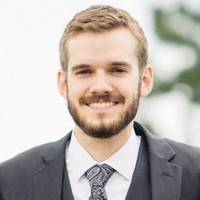
\includegraphics{headshot.jpeg}

\textbf{UPDATE: I will be departing DataRobot in April 2020, and am in
the market for new opportunities, preferably in the DC/Baltimore area,
or remote friendly. I am willing to obtain a clearance (no active,
previously held public trust), and travel up to 50\%.}

\begin{wrapfig}[12]{l}[2pt]{5cm}
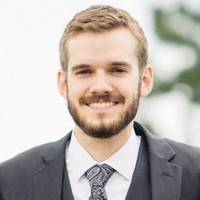
\includegraphics[width=0.25\textwidth]{headshot.jpeg}
\end{wrapfig}

Paul is an experienced data scientist, programmer, consultant, and team
leader. He specializes in bringing powerful machine learning models into
real situations quickly and practically, with a focus on value and
impact. He has served clients from several industries, including
government, non-profit, and healthcare.

In addition to a strong foundation in math and statistics, Paul has 8
years of programming experience in a wide variety of languages,
including C++, Java, SAS, SQL, and especially Python and R. He is also
comfortable with industry-standard tools used in the data science
pipeline such as Linux, Git, AWS and Agile processes. He has several
years of experience leading small teams and mentoring junior data
scientists.

Paul is completing his Masters in Computer Science through the Johns
Hopkins Whiting School of Engineering this Summer. He is a Customer
Facing Data Scientist for DataRobot's AI for Good pro bono program for
organizations with a large social impact.

Paul grew up in Denver, CO, and graduated from the University of
Colorado at Boulder with degrees in Applied Math and Economics Magna cum
laude in 2012. He lives with his wife and pet beagle in Jessup, MD,
between Washington and Baltimore. He is an avid skier, hobbyist
musician, and aspiring home-improvement DIYer.


\end{document}
